\section{Metodología}
\label{sec:metodologia}

En esta sección se detalla el marco metodológico integral adoptado para el modelado físico-electromagnético, el diseño y dimensionamiento circuital de las etapas de transmisión (TX) y recepción (RX), el protocolo de comunicación digital en microcontroladores ESP32 y el análisis paramétrico comparativo entre los inductores comerciales nominales y el electroimán experimental implementado en laboratorio.

\subsection{Modelo Físico y Formulación Electromagnética}
\label{subsec:modelo_fisico}

El enlace se modela como dos bobinas magnéticamente acopladas en un medio homogéneo y no magnético ($\mu \approx \mu_0$).

\subsubsection{Distribución de Inducción Magnética (Ley de Biot-Savart)}
Para una bobina circular transmisora de radio medio $a$, conformada por $N_1$ espiras recorridas por una corriente armónica $i_1(t)$, la ley de Biot-Savart establece que la densidad de flujo magnético axial a una distancia $z$ sobre el eje normal al plano de la espira está dada por~\cite{hayt2012electromagnetics}:
\begin{equation}
    B_z(z, t) = \frac{\mu_0 N_1 i_1(t) a^2}{2 (a^2 + z^2)^{3/2}}
    \label{eq:biot_savart}
\end{equation}
donde $\mu_0 = 4\pi \times 10^{-7}\text{ H/m}$ representa la permeabilidad magnética del vacío.

Para distancias axiales sensiblemente superiores al radio físico de la bobina ($z \gg a$), la ecuación~(\ref{eq:biot_savart}) converge asintóticamente al modelo de dipolo magnético puntual:
\begin{equation}
    B_z(z, t) \approx \frac{\mu_0 m(t)}{2\pi z^3}
    \label{eq:dipolo_magnetico}
\end{equation}
donde $m(t) = N_1 i_1(t) \pi a^2$ es el momento dipolar magnético. La ecuación~(\ref{eq:dipolo_magnetico}) demuestra la atenuación geométrica de tercer orden ($1/z^3$) de la densidad de flujo en campo reactivo~\cite{finkenzeller2010rfid}.

\subsubsection{Flujo Concatenado, Inductancia Mutua y Factor de Acoplamiento}
El flujo magnético concatenado $\Phi_{21}(z, t)$ por una bobina receptora coaxial de $N_2$ espiras y superficie transversal $S_2$ ubicada a distancia $z$ resulta de integrar $B_z$ sobre dicha superficie:
\begin{equation}
    \Phi_{21}(z, t) \approx B_z(z, t) \cdot S_2 = \frac{\mu_0 N_1 S_2 a^2}{2 (a^2 + z^2)^{3/2}} i_1(t)
    \label{eq:flujo_concatenado}
\end{equation}
La inductancia mutua $M(z)$ se define como la razón entre el flujo total enlazado y la corriente primaria:
\begin{equation}
    M(z) = \frac{N_2 \Phi_{21}(z, t)}{i_1(t)} = \frac{\mu_0 N_1 N_2 S_1 S_2}{2\pi (a^2 + z^2)^{3/2}}
    \label{eq:inductancia_mutua}
\end{equation}
El factor de acoplamiento magnético adimensional $k(z)$ normaliza la inductancia mutua respecto a las autoinductancias propias $L_1$ y $L_2$~\cite{lee2003antenna}:
\begin{equation}
    k(z) = \frac{M(z)}{\sqrt{L_1 L_2}}, \quad 0 \le k(z) < 1
    \label{eq:factor_acoplamiento}
\end{equation}

\subsubsection{Fuerza Electromotriz Inducida (Ley de Faraday-Lenz)}
Conforme a la ley de Faraday-Lenz, la fuerza electromotriz inducida ($\mathcal{E}_{\text{ind}}$) en bornes del inductor receptor en circuito abierto es:
\begin{equation}
    \mathcal{E}_{\text{ind}}(t) = - M(z) \frac{d i_1(t)}{dt}
    \label{eq:faraday}
\end{equation}
Bajo excitación armónica sinusoidal $i_1(t) = I_{1,\text{pk}} \cos(\omega_0 t)$ con pulsación angular $\omega_0 = 2\pi f_0$:
\begin{equation}
    \mathcal{E}_{\text{ind}}(t) = \omega_0 M(z) I_{1,\text{pk}} \sin(\omega_0 t)
    \label{eq:fem_armonica}
\end{equation}

\subsubsection{Topología Resonante Asimétrica}
Para superar la atenuación cúbica y optimizar la relación señal a ruido (SNR), ambas etapas se sintonizan a la portadora mediante redes LC resonantes:
\begin{equation}
    f_0 = \frac{1}{2\pi \sqrt{L C_{\text{res}}}} = \SI{125.04}{\kilo\hertz}
    \label{eq:frecuencia_resonancia}
\end{equation}
\begin{itemize}
    \item \textbf{Tanque Transmisor Serie ($L_1$ en serie con $C_{\text{res}}$):} En resonancia ($\omega = \omega_0$), la reactancia inductiva y capacitiva se cancelan ($X_{L1} = X_C$), reduciéndose la impedancia vista por el excitador a su componente puramente resistiva mínima:
    \begin{equation}
        Z_{\text{TX}}(\omega_0) = R_{\text{total}} = R_{\text{limit}} + R_{\text{ESR}} + R_{DS(\text{on})}
        \label{eq:ztx_min}
    \end{equation}
    Esto permite inyectar la máxima corriente en la bobina emisora ($I_{\text{pk}} \propto 1/R_{\text{total}}$), maximizando el momento dipolar.
    \item \textbf{Tanque Receptor Paralelo ($L_2$ en paralelo con $C_{\text{res}}$):} Presenta impedancia máxima a la resonancia, actuando como un multiplicador pasivo de tensión. La tensión en bornes del tanque en circuito abierto se amplifica respecto a la FEM inducida por el factor de calidad no cargado $Q_0$:
    \begin{equation}
        V_{\text{tank}}(\omega_0) \approx Q_0 \cdot \mathcal{E}_{\text{ind}} = \left( \frac{\omega_0 L_2}{R_{\text{ESR}}} \right) \mathcal{E}_{\text{ind}}
        \label{eq:ganancia_q_pasiva}
    \end{equation}
\end{itemize}

\subsection{Análisis Paramétrico: Inductor Comercial vs. Electroimán de Laboratorio}
\label{subsec:analisis_inductor_fallo}

Durante la fase preliminar de evaluación experimental, ante la indisponibilidad temporal de bobinas comerciales de \SI{1.0}{\milli\henry}, se construyó un inductor experimental casero tipo electroimán. El análisis electromagnético cuantitativo de este elemento explica matemáticamente el colapso del enlace observado en el laboratorio:

\begin{enumerate}
    \item \textbf{Geometría del Núcleo y Bobinado:} Se utilizó un núcleo de ferrita rectangular de longitud $\ell_c = \SI{3.5}{\centi\meter} = \SI{35}{\milli\meter}$, ancho $w = \SI{0.5}{\centi\meter} = \SI{5}{\milli\meter}$ y altura $h = \SI{1.3}{\centi\meter} = \SI{13}{\milli\meter}$. El área transversal de la sección magnética es:
    \begin{equation}
        S_{\text{core}} = w \times h = 5 \times 13 = \SI{65}{\milli\meter\squared} = \SI{6.5e-5}{\meter\squared}
    \end{equation}
    El bobinado se extendió a lo largo de $\ell_w = \SI{2.6}{\centi\meter} = \SI{26}{\milli\meter}$ utilizando alambre de cobre esmaltado de diámetro $d_{\text{cu}} = \SI{0.1}{\centi\meter} = \SI{1.0}{\milli\meter}$.
    \item \textbf{Número de Espiras Efectivas:} Debido al grosor del alambre ($1.0\text{ mm}$), el número máximo de espiras que pueden acomodarse en una sola capa es:
    \begin{equation}
        N_1 = \left\lfloor \frac{\ell_w}{d_{\text{cu}}} \right\rfloor = \frac{\SI{26}{\milli\meter}}{\SI{1.0}{\milli\meter}} \approx 26 \text{ espiras}
    \end{equation}
    (oscilando entre 26 y 30 espiras considerando espiras de cierre). Esto contrasta frontalmente con una bobina comercial RFID LF de \SI{1.0}{\milli\henry}, que integra entre 350 y 500 espiras de alambre ultrafino (AWG 38--40, $d \approx \SI{0.08}{\milli\meter}$).
    \item \textbf{Permeabilidad Aparente de Barra Desmagnetizada:} Para una barra abierta de ferrita con relación de aspecto $p = \ell_c / d_{\text{eq}} \approx 35 / 9.1 \approx 3.85$, el factor de desmagnetización geométrico ($D \approx 0.05$) reduce la permeabilidad relativa efectiva a:
    \begin{equation}
        \mu_{\text{app}} = \frac{\mu_r}{1 + D (\mu_r - 1)} \approx 18 - 22 \approx 20
    \end{equation}
    \item \textbf{Inductancia Resultante:} La autoinductancia del electroimán casero resulta:
    \begin{equation}
        L_{\text{exp}} = \mu_0 \mu_{\text{app}} \frac{N^2 S_{\text{core}}}{\ell_w} \approx (4\pi \times 10^{-7}) (20) \frac{26^2 (\num{6.5e-5})}{0.026} \approx \SI{42.5}{\micro\henry}
    \end{equation}
    Es decir, **23.5 veces inferior** al valor de diseño nominal ($L_{\text{nom}} = \SI{1000}{\micro\henry}$).
    \item \textbf{Desintonización Resonante Catastrófica:} Al conectarse al banco capacitivo de sintonía ($C_{\text{res}} = \SI{1.62}{\nano\farad}$), la frecuencia natural de resonancia se desplazó a:
    \begin{equation}
        f_0' = \frac{1}{2\pi \sqrt{L_{\text{exp}} C_{\text{res}}}} = \frac{1}{2\pi \sqrt{(\num{42.5e-6})(\num{1.62e-9})}} \approx \SI{607.4}{\kilo\hertz}
    \end{equation}
    desfasándose en casi medio megahercio respecto a los \SI{125}{\kilo\hertz} del oscilador.
    \item \textbf{Colapso de Impedancia en TX:} A la frecuencia de trabajo de \SI{125}{\kilo\hertz}:
    \begin{equation}
        X_L = \omega L_{\text{exp}} = 2\pi (125000)(\num{42.5e-6}) \approx \SI{33.4}{\ohm}
    \end{equation}
    \begin{equation}
        X_C = \frac{1}{\omega C_{\text{res}}} = \frac{1}{2\pi (125000)(\num{1.62e-9})} \approx \SI{785.6}{\ohm}
    \end{equation}
    La impedancia total vista por el driver TC4427A deja de ser mínima y pasa a ser fuertemente capacitiva:
    \begin{equation}
        |Z_{\text{TX}}(125\text{ kHz})| = \sqrt{R_{\text{limit}}^2 + (X_L - X_C)^2} \approx \sqrt{150^2 + (-752.2)^2} \approx \SI{767.0}{\ohm}
    \end{equation}
    La corriente fundamental inyectada a la bobina se redujo a:
    \begin{equation}
        I_{\text{TX,exp}} = \frac{V_{1,\text{pk}}}{|Z_{\text{TX}}|} = \frac{\SI{3.183}{\volt}}{\SI{767.0}{\ohm}} \approx \SI{4.15}{\milli\ampere}
    \end{equation}
    \item \textbf{Atenuación del Momento Dipolar Magnético:} El momento magnético radiado por el electroimán experimental fue de apenas:
    \begin{equation}
        m_{\text{exp}} = N I_{\text{TX,exp}} S_{\text{core}} = 26 \times (\num{4.15e-3}) \times (\num{6.5e-5}) \approx \SI{7.01e-6}{\ampere\meter\squared}
    \end{equation}
    Frente al diseño nominal ($m_{\text{nom}} \approx \SI{5.50e-3}{\ampere\meter\squared}$), la emisión magnética sufrió una atenuación de:
    \begin{equation}
        \frac{m_{\text{exp}}}{m_{\text{nom}}} \approx \frac{\num{7.01e-6}}{\num{5.50e-3}} \approx \num{1.27e-3} \quad (\SI{-57.9}{\deci\bel})
    \end{equation}
    \item \textbf{Efecto Cortocircuito en Recepción:} En el tanque receptor paralelo, una reactancia de solo $X_L \approx \SI{33.4}{\ohm}$ a \SI{125}{\kilo\hertz} deriva directamente a masa cualquier fuerza electromotriz inducida. El factor de calidad se reduce a $Q \ll 1$, imposibilitando cualquier elevación pasiva de tensión y provocando una señal nula en el detector.
\end{enumerate}

\subsection{Diseño y Topología de Circuitos Hardware}
\label{subsec:diseno_circuitos}

El hardware implementado integra dos módulos físicamente independientes gobernados por microcontroladores ESP32 DevKitC: el transmisor (TX, \SI{5}{\volt}) y el receptor (RX, \SI{3.3}{\volt}).

\subsubsection{Etapa Transmisora (TX)}
Consta de cuatro bloques funcionales:
\begin{enumerate}
    \item \textbf{Generador de Portadora (TLC555):} Temporizador astable calibrado a \SI{125}{\kilo\hertz} mediante $R_A = \SI{4.7}{\kilo\ohm}$, potenciómetro $RV_1 = \SI{10}{\kilo\ohm}$ con resistencia de seguridad de \SI{1}{\kilo\ohm} y $C_1 = \SI{1}{\nano\farad}$.
    \item \textbf{Modulación OOK Activa por Gating:} La señal digital de datos del pin \texttt{GPIO18} gobierna directamente el pin \texttt{\textasciitilde RST} (pin 4) del TLC555. El nivel alto (\SI{3.3}{\volt}) habilita la oscilación libre y el nivel bajo (\SI{0}{\volt}) bloquea el oscilador instantáneamente en estado bajo.
    \item \textbf{Driver de Potencia (TC4427A):} Buffer MOSFET dual (\SI{1.5}{\ampere} pico, $t_r = \SI{20}{\nano\second}$), alimentado a \SI{5}{\volt}, excitando el tanque resonante serie. El canal B no utilizado se conecta a masa para evitar oscilaciones parásitas.
    \item \textbf{Tanque Resonante Serie TX:} Resistor de límite $R_{\text{limit}} = \SI{150}{\ohm}$, inductor LF $L_1 = \SI{1.0}{\milli\henry}$ ($R_{\text{ESR}} \approx \SI{10}{\ohm}$) y capacitores C0G en paralelo ($1.5\text{ nF} \parallel 120\text{ pF} = \SI{1.62}{\nano\farad}$).
\end{enumerate}

\begin{figure}[htbp]
\centering
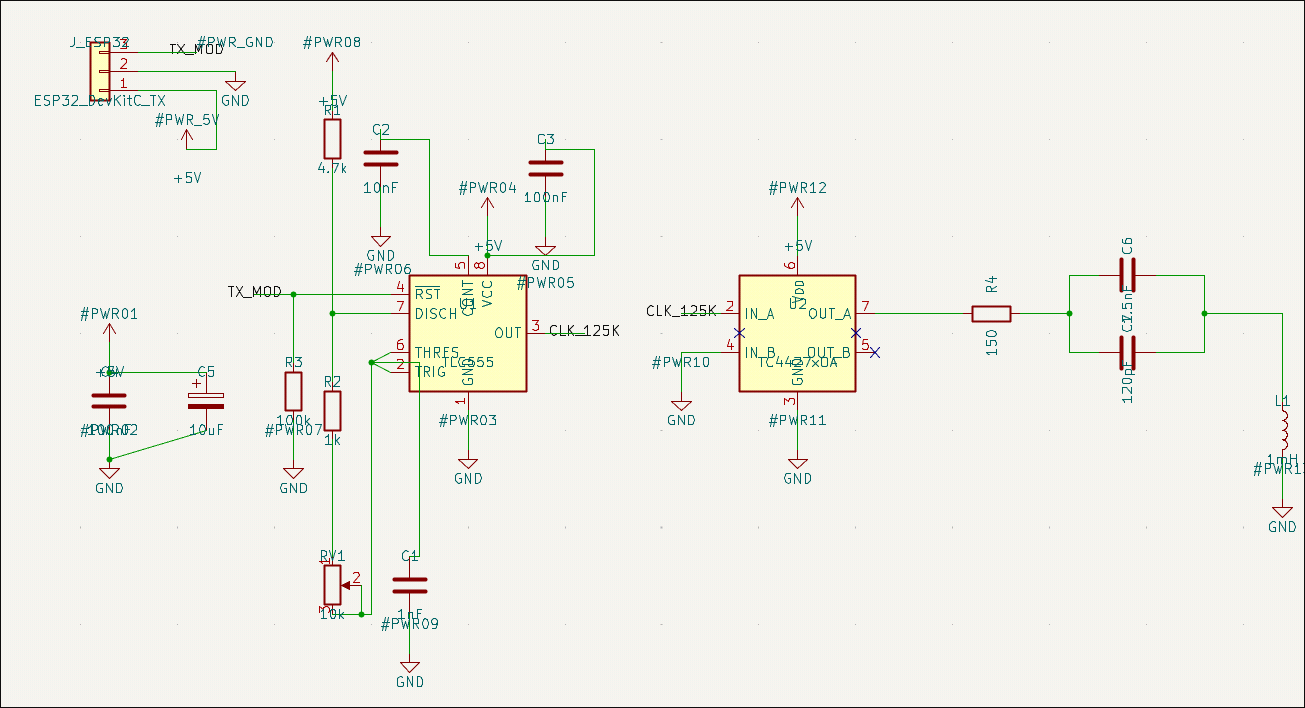
\includegraphics[width=0.98\columnwidth]{circuito_tx_esquematico.png}
\caption{Esquema circuital del transmisor (TX): conector ESP32 DevKitC, oscilador astable TLC555 con modulación OOK por control de pin \texttt{\textasciitilde RST}, driver MOSFET push-pull TC4427A alimentado a \SI{5}{\volt} y red de resonancia serie ($L_1 = \SI{1.0}{\milli\henry}$, $C_6 = 1.5\text{ nF} \parallel 120\text{ pF}$, $R_4 = \SI{150}{\ohm}$).}
\label{fig:circuito_tx}
\end{figure}

\subsubsection{Etapa Receptora (RX)}
Acondiciona señales captadas de milivoltios bajo un riel monofuente de \SI{3.3}{\volt}:
\begin{enumerate}
    \item \textbf{Tanque Paralelo y Masa Virtual:} Bobina $L_2 = \SI{1.0}{\milli\henry}$ en paralelo con $C_{\text{res}} = \SI{1.62}{\nano\farad}$, polarizada a una masa virtual fija $V_{\text{ref}} = \SI{1.65}{\volt}$ provista por un divisor resistivo desacoplado ($2 \times \SI{100}{\kilo\ohm} + \SI{1}{\micro\farad} + \SI{100}{\nano\farad}$).
    \item \textbf{Preamplificador en Cascada (MCP6002):} Dos etapas inversoras Rail-to-Rail:
    \begin{itemize}
        \item Etapa 1: $R_{\text{in1}} = \SI{10}{\kilo\ohm}$, $R_{f1} = \SI{68}{\kilo\ohm} \implies A_{v1,\text{DC}} = -6.8$.
        \item Etapa 2: $R_{\text{in2}} = \SI{10}{\kilo\ohm}$, $R_{f2} = \SI{47}{\kilo\ohm} \implies A_{v2,\text{DC}} = -4.7$.
    \end{itemize}
    \item \textbf{Desacoplo AC y Demodulador de Envolvente:} Red de paso alto ($C_7 = \SI{100}{\nano\farad}$, $R_{12} = \SI{100}{\kilo\ohm}$) que remueve la continua de \SI{1.65}{\volt}. El diodo Schottky BAT85 ($V_F \approx \SI{0.25}{\volt}$) rectifica la señal hacia un filtro pasa-bajos RC ($R_7 = \SI{100}{\kilo\ohm}$, $C_6 = \SI{10}{\nano\farad}$, $\tau = \SI{1.0}{\milli\second}$).
    \item \textbf{Conformador con Histéresis (LM393):} Comparador con umbral $V_{\text{th}} \approx \SI{0.30}{\volt}$ fijado por divisor resistivo e histéresis positiva con $R_{10} = \SI{1}{\mega\ohm}$ para inmunidad contra rebotes parásitos, conectado al pin \texttt{GPIO19} del ESP32.
\end{enumerate}

\begin{figure}[htbp]
\centering
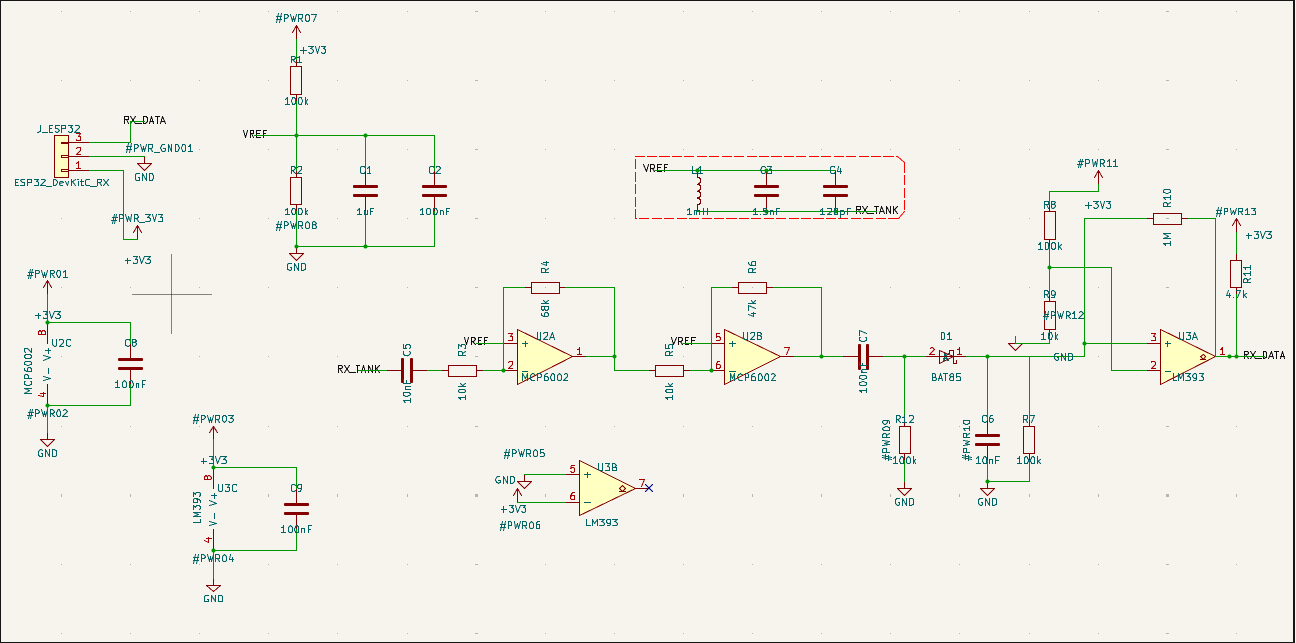
\includegraphics[width=0.98\columnwidth]{circuito_rx_esquematico.png}
\caption{Esquema circuital del receptor (RX): polarización de masa virtual ($V_{\text{ref}} = \SI{1.65}{\volt}$), tanque LC paralelo sintonizado, amplificación en dos etapas inversoras con MCP6002, filtro demodulador de envolvente con diodo Schottky BAT85 y conformador digital LM393 con histéresis.}
\label{fig:circuito_rx}
\end{figure}

\begin{table}[htbp]
\caption{BOM y Comparación de Inductores del Proyecto}
\label{tab:componentes}
\centering
\begin{tabular}{llcc}
\toprule
\textbf{Parámetro / Componente} & \textbf{Nominal Diseño} & \textbf{Electroimán Lab.} & \textbf{Unidad} \\
\midrule
Inductancia ($L$) & \num{1.0} & \num{0.0425} & \si{\milli\henry} \\
Número de espiras ($N$) & $\approx 400$ & $\approx 26-30$ & espiras \\
Diámetro alambre ($d_{\text{cu}}$) & \num{0.08} (AWG 40) & \num{1.0} (AWG 18) & \si{\milli\meter} \\
Sección núcleo ($S$) & $\approx 70.7$ (circular) & \num{65.0} (rectangular) & \si{\milli\meter\squared} \\
Capacitor de sintonía ($C_{\text{res}}$) & \num{1.62} & \num{1.62} & \si{\nano\farad} \\
Frecuencia resonancia ($f_0$) & \textbf{125.04} & \textbf{607.4} & \si{\kilo\hertz} \\
Reactancia $X_L$ a \SI{125}{\kilo\hertz} & \num{785.65} & \num{33.4} & \si{\ohm} \\
Impedancia TX $|Z_{\text{TX}}|$ & \num{163.50} & \num{767.0} & \si{\ohm} \\
Corriente pico TX ($I_{\text{pk}}$) & \num{19.47} & \num{4.15} & \si{\milli\ampere} \\
Momento dipolar ($m$) & \num{5.50e-3} & \num{7.01e-6} & \si{\ampere\meter\squared} \\
Atenuación relativa de $m$ & $0.0$ & \textbf{-57.9} & \si{\deci\bel} \\
Estado del enlace de datos & \textbf{Operativo (PER=0)} & \textbf{Fallo Total (CH2=0V)} & -- \\
\bottomrule
\end{tabular}
\end{table}

\subsection{Protocolo de Comunicación y Firmware en Microcontrolador}
\label{subsec:firmware}

El microcontrolador ESP32 implementa codificación Manchester IEEE 802.3 a \SI{250}{\text{bps}}:
\begin{itemize}
    \item \textbf{Temporización por Hardware:} Temporizador de precisión de microsegundos de ESP-IDF (\texttt{esp\_timer}) a \SI{500}{\hertz} ($T_{\text{half}} = \SI{2000}{\micro\second}$).
    \item \textbf{Decodificación por Interrupciones y Filtrado Anti-Glitch:} En recepción, el pin \texttt{GPIO19} detecta flancos por interrupción (\texttt{IRAM\_ATTR isr\_rx\_edge}). Un discriminador temporal descarta pulsos espurios menores a \SI{600}{\micro\second} con ventana de aceptación de $\pm 25\%$.
    \item \textbf{Estructura de Trama:} Preámbulo de sincronización (\texttt{0xAA}, 2 bytes), delimitador SFD (\texttt{0x7E}, 1 byte), longitud $N$ (1 byte, $1 \le N \le 32$), carga útil ($N$ bytes) y checksum CRC-8 con polinomio $P(x) = x^8 + x^2 + x + 1$ (\texttt{0x07}, 1 byte).
\end{itemize}
